\documentclass[11pt,a4paper]{article}

% ---------------------------------------------------------------- packages
\usepackage[T1]{fontenc}
\usepackage[utf8]{inputenc}
\usepackage{libertinus}
\usepackage[scaled=0.86]{sourcecodepro}
\usepackage[margin=2.15cm,top=2.3cm,bottom=2.3cm]{geometry}
\usepackage{amsmath,amssymb}
\usepackage{booktabs}
\usepackage{array}
\usepackage{xcolor}
\usepackage{graphicx}
\usepackage{listings}
\usepackage{enumitem}
\usepackage{titlesec}
\usepackage{tcolorbox}
\usepackage{tikz}
\usepackage{microtype}
\usepackage{caption}
\usepackage{fancyhdr}
\usepackage{multicol}
\usepackage[hidelinks,colorlinks=true,linkcolor=accent,urlcolor=accent]{hyperref}
\usetikzlibrary{arrows.meta,positioning,fit,backgrounds}
\tcbuselibrary{skins,breakable}

% ------------------------------------------------------------------ colours
\definecolor{accent}{HTML}{2A78D6}
\definecolor{accent2}{HTML}{EB6834}
\definecolor{aqua}{HTML}{1BAF7A}
\definecolor{ink}{HTML}{0B0B0B}
\definecolor{ink2}{HTML}{52514E}
\definecolor{ink3}{HTML}{8A8983}
\definecolor{rule}{HTML}{E3E2DD}
\definecolor{surf}{HTML}{FAFAF8}
\definecolor{surf2}{HTML}{F0EFEC}

% ------------------------------------------------------------------ styling
\titleformat{\section}{\normalfont\Large\bfseries\color{accent}}{\thesection}{0.7em}{}
\titleformat{\subsection}{\normalfont\large\bfseries\color{ink}}{\thesubsection}{0.6em}{}
\titleformat{\subsubsection}{\normalfont\normalsize\bfseries\color{ink2}}{\thesubsubsection}{0.6em}{}
\titlespacing*{\section}{0pt}{1.6em}{0.7em}
\titlespacing*{\subsection}{0pt}{1.1em}{0.45em}

\captionsetup{font=small,labelfont={bf,color=accent},textfont={color=ink2}}
\captionsetup{justification=raggedright,singlelinecheck=false}
\renewcommand{\arraystretch}{1.25}
\setlength{\parindent}{0pt}
\setlength{\parskip}{0.5em}
% Inline \code{...} spans are unbreakable monospace, so a long one at the end of
% a line has nowhere to go. Give TeX slack instead of an overfull box.
\sloppy
\setlength{\emergencystretch}{3em}

\pagestyle{fancy}
\fancyhf{}
\renewcommand{\headrulewidth}{0.4pt}
\renewcommand{\headrule}{\hbox to\headwidth{\color{rule}\leaders\hrule height \headrulewidth\hfill}}
\fancyhead[L]{\small\color{ink3}Drift Field Inference \textemdash{} Framework Reference}
\fancyfoot[C]{\small\color{ink3}\thepage}

% ------------------------------------------------------------------ listings
\lstdefinestyle{py}{
  language=Python,
  basicstyle=\ttfamily\footnotesize\color{ink},
  keywordstyle=\color{accent}\bfseries,
  commentstyle=\color{ink3}\itshape,
  stringstyle=\color{aqua},
  numberstyle=\tiny\color{ink3},
  showstringspaces=false,
  breaklines=true,
  breakatwhitespace=true,
  frame=none,
  columns=fullflexible,
  keepspaces=true,
  upquote=true,
  aboveskip=0.6em, belowskip=0.4em,
}
\lstset{style=py}

\newtcolorbox{codebox}{
  enhanced, breakable, colback=surf2, colframe=rule, boxrule=0.5pt,
  arc=2pt, left=7pt, right=7pt, top=5pt, bottom=5pt, boxsep=0pt
}
\newtcolorbox{keybox}[1][]{
  enhanced, breakable, colback=accent!5, colframe=accent, boxrule=0pt,
  leftrule=2.5pt, arc=0pt, left=9pt, right=9pt, top=6pt, bottom=6pt, #1
}
\newtcolorbox{warnbox}[1][]{
  enhanced, breakable, colback=accent2!6, colframe=accent2, boxrule=0pt,
  leftrule=2.5pt, arc=0pt, left=9pt, right=9pt, top=6pt, bottom=6pt, #1
}

\newcommand{\code}[1]{{\ttfamily\small #1}}
\newcommand{\bt}[1]{{\ttfamily\footnotesize #1}}
\newcommand{\yours}{{\color{accent2}\footnotesize\bfseries YOURS}}
\newcommand{\built}{{\color{aqua}\footnotesize\bfseries BUILT}}

\newcolumntype{L}[1]{>{\raggedright\arraybackslash}p{#1}}
\newcolumntype{C}[1]{>{\centering\arraybackslash}p{#1}}

% ==========================================================================
\begin{document}

% ------------------------------------------------------------- title block
\begin{center}
{\LARGE\bfseries\color{ink} Recovering Drift Fields from Random Walks}\\[0.35em]
{\Large\color{accent} Framework Reference}\\[1.0em]
{\color{ink2}\large The \code{dfi} package: data you can create, estimators you can plug in,\\
and the measurements that compare them}\\[1.2em]
{\color{ink3}\small Version 0.1 \quad\textbullet\quad 6\,600 lines \quad\textbullet\quad 28 tests passing}
\end{center}

\vspace{0.6em}
\hrule height 0.4pt \vspace{1.2em}

\begin{keybox}
\textbf{What this document is.} A reference for the parts of the project that are
already built and tested: how to \emph{generate} flow fields, how to \emph{simulate}
walkers in them, what \emph{data objects} come out, what \emph{contract} an estimator
must satisfy, and how errors are \emph{measured} and \emph{plotted}. The five
estimators themselves are specified here but left unimplemented \textemdash{} they are
yours to write. Sections marked \built{} work now; sections marked \yours{} are stubs
with full specifications.
\end{keybox}

\vspace{0.4em}
{\small\color{ink2}
\setlength{\parskip}{0pt}
\begin{multicols}{2}
\tableofcontents
\end{multicols}}

\clearpage

% ==========================================================================
\section{The problem}

We observe particles obeying the overdamped Langevin equation
\begin{equation}
  \mathrm{d}x = b(x)\,\mathrm{d}t + \sqrt{2D}\,\mathrm{d}W ,
  \label{eq:sde}
\end{equation}
whose density evolves by the Fokker\textendash{}Planck equation
$\partial_t\rho = -\nabla\!\cdot\!(b\rho) + D\nabla^2\rho$.
The inverse problem is to recover the vector field $b(x)$ from observed motion.

There are two fundamentally different data regimes, and keeping them apart is the
scientific spine of the project.

\begin{center}
\begin{tabular}{@{}L{0.46\textwidth} L{0.46\textwidth}@{}}
\toprule
\textbf{(a) Trajectories} & \textbf{(b) Snapshots} \\
\midrule
Positions \emph{with} time ordering, sampled at spacing $\Delta t$.
The Kramers\textendash{}Moyal estimator is a local conditional average,
\[ b(x)\approx\tfrac{1}{\Delta t}\,\mathbb{E}\!\left[\Delta x \mid x\right]. \]
Can recover \emph{all} of $b$.
&
Unordered positions drawn from $\rho_{\mathrm{ss}}$. The only recoverable object is the
score,
\[ \nabla\log\rho_{\mathrm{ss}} = -\nabla U/D . \]
Can recover \emph{only} the gradient part.
\\
\bottomrule
\end{tabular}
\end{center}

\begin{keybox}
\textbf{The identifiability gap.} Split the drift into a curl-free and a
divergence-free part, $b = -\nabla U + b_{\mathrm{rot}}$. The rotational component
carries a steady probability current but leaves $\rho_{\mathrm{ss}}$ \emph{unchanged}.
So a snapshot dataset is \emph{literally identical in distribution} for a system with
no circulation and one with a great deal of it. This is not a weakness of any
particular method; the information is absent from the data. Demonstrating it
quantitatively is the project's headline result.
\end{keybox}

% ==========================================================================
\section{The framework at a glance}

\begin{center}
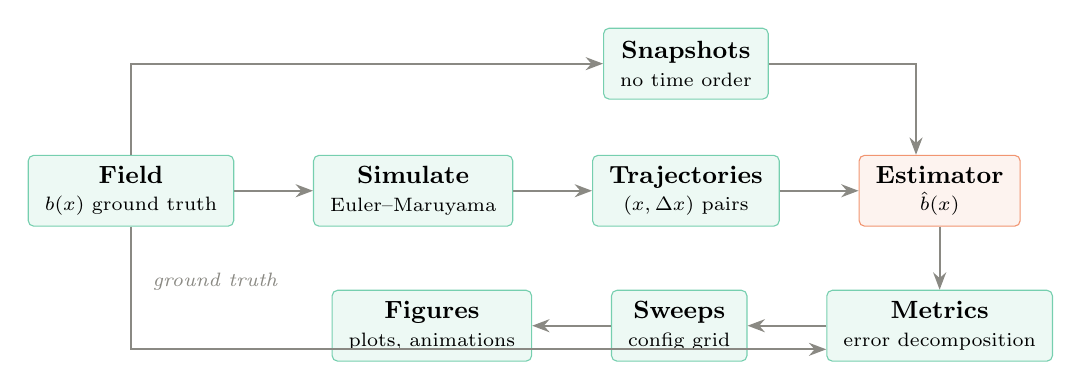
\begin{tikzpicture}[
  node distance=6mm,
  box/.style={draw=rule, fill=surf2, rounded corners=2pt, minimum height=9mm,
              inner xsep=6pt, font=\small, align=center},
  built/.style={box, draw=aqua!60, fill=aqua!8},
  yours/.style={box, draw=accent2!70, fill=accent2!8},
  arr/.style={-{Stealth[length=2.2mm]}, draw=ink3, thick}
]
\node[built] (field) {\textbf{Field}\\[-1pt]{\scriptsize $b(x)$ ground truth}};
\node[built, right=10mm of field] (sim) {\textbf{Simulate}\\[-1pt]{\scriptsize Euler\textendash{}Maruyama}};
\node[built, right=10mm of sim] (data) {\textbf{Trajectories}\\[-1pt]{\scriptsize $(x,\Delta x)$ pairs}};
\node[yours, right=10mm of data] (est) {\textbf{Estimator}\\[-1pt]{\scriptsize $\hat b(x)$}};
\node[built, below=8mm of est] (met) {\textbf{Metrics}\\[-1pt]{\scriptsize error decomposition}};
\node[built, left=10mm of met] (swp) {\textbf{Sweeps}\\[-1pt]{\scriptsize config grid}};
\node[built, left=10mm of swp] (viz) {\textbf{Figures}\\[-1pt]{\scriptsize plots, animations}};
\node[built, above=7mm of data] (snap) {\textbf{Snapshots}\\[-1pt]{\scriptsize no time order}};

\draw[arr] (field) -- (sim);
\draw[arr] (sim) -- (data);
\draw[arr] (data) -- (est);
\draw[arr] (est) -- (met);
\draw[arr] (met) -- (swp);
\draw[arr] (swp) -- (viz);
\draw[arr] (field.north) |- (snap.west);
\draw[arr] (snap.east) -| ([xshift=-3mm]est.north);
\draw[arr] (field.south) |- ([yshift=-3mm]met.west);
\node[font=\scriptsize\itshape, color=ink3, anchor=west]
      at ([xshift=1.5mm,yshift=-7mm]field.south) {ground truth};
\end{tikzpicture}
\end{center}

\vspace{-0.6em}
\begin{center}
{\footnotesize\color{ink3}Green = built and tested \quad\textbullet\quad Orange = your implementation}
\end{center}

\subsection{Module map}

\begin{center}
\begin{tabular}{@{}L{0.30\textwidth} L{0.55\textwidth} C{0.08\textwidth}@{}}
\toprule
\textbf{Module} & \textbf{Contents} & \textbf{Status} \\
\midrule
\bt{dfi/fields/domain.py}       & \code{Box}: torus or open box, minimum-image displacement & \built \\
\bt{dfi/fields/noise.py}        & Gaussian random fields, Perlin/fBm, spectral derivatives & \built \\
\bt{dfi/fields/base.py}         & \code{DriftField} interface, Helmholtz split, antisymmetric $A$ & \built \\
\bt{dfi/fields/random\_field.py}& \code{GridDriftField}, \code{SpectralDriftField} & \built \\
\bt{dfi/fields/analytic.py}     & OU, coupled chain, double well, radial+rotational & \built \\
\bt{dfi/simulate.py}            & Euler\textendash{}Maruyama, numpy + torch/GPU, step diagnostics & \built \\
\bt{dfi/trajectories.py}        & \code{Trajectories} container, reshaping, diagnostics & \built \\
\bt{dfi/estimators/base.py}     & Estimator contract, registry, \code{ZeroDrift}/\code{OracleDrift} & \built \\
\bt{dfi/estimators/local.py}    & Rungs 1\textendash{}2: binned KM, kernel regression & \yours \\
\bt{dfi/estimators/basis.py}    & Rung 3: basis projection (SFI) + error bound & \yours \\
\bt{dfi/estimators/neural.py}   & Rung 4: MLP regression & \yours \\
\bt{dfi/estimators/score.py}    & Rung 5: KDE score, denoising score matching & \yours \\
\bt{dfi/metrics.py}             & Evaluation sets, error decomposition, error vs density & \built \\
\bt{dfi/sweeps.py}              & Config grid runner with caching and resume & \built \\
\bt{dfi/viz/}                   & Style tokens, LIC textures, all plots and animations & \built \\
\bottomrule
\end{tabular}
\end{center}

% ==========================================================================
\clearpage
\section{Data you can create}

This is the part of the framework you drive directly. Three kinds of object:
\textbf{fields} (the ground truth), \textbf{trajectories} (time-ordered observations),
and \textbf{snapshots} (unordered samples).

\subsection{The construction behind every random field}

All random fields are built from a \emph{scalar} potential, never from two independent
noise vector fields:
\begin{equation}
  \boxed{\;b(x) \;=\; -\nabla U(x) \;+\; \omega\,A\,\nabla U(x)\;}
  \qquad A^{\mathsf T} = -A,\ \ A \text{ constant}.
  \label{eq:construction}
\end{equation}

\begin{keybox}
\textbf{Why this exact form.} Two identities hold \emph{pointwise and exactly}:
\[
  \nabla\!\cdot\!(A\nabla U) = A_{ij}\,\partial_i\partial_j U = 0,
  \qquad
  \nabla U \cdot A\nabla U = 0 ,
\]
the first because an antisymmetric matrix contracted with the symmetric Hessian
vanishes, the second because an antisymmetric quadratic form vanishes. So the second
term is genuinely divergence-free \emph{and} everywhere orthogonal to
$\nabla\rho_{\mathrm{ss}}$. Substituting $\rho = e^{-U/D}$ into Fokker\textendash{}Planck
leaves the residual current $J = \omega\,(A\nabla U)\,\rho$, which is divergence free.

\textbf{Consequences, all free:}
\begin{itemize}[leftmargin=1.2em,itemsep=1pt,topsep=2pt]
  \item the Helmholtz decomposition is \emph{exact}, not estimated;
  \item $\rho_{\mathrm{ss}} = e^{-U/D}/Z$ is exact \textbf{for every} $\omega$
        (verified: Fokker\textendash{}Planck residual $2\times10^{-7}$);
  \item \code{field.with\_omega(w)} changes the dynamics while holding
        $\rho_{\mathrm{ss}}$ \emph{bit-identical} \textemdash{} the airtight
        identifiability experiment;
  \item $\omega$ reads directly as the rotational-to-gradient amplitude ratio;
  \item it works in \emph{any} dimension (in 2D, $A$ is the perpendicular gradient);
  \item in $d=1$, $A$ is necessarily zero \textemdash{} correctly, since no
        divergence-free field exists on a line.
\end{itemize}
\end{keybox}

\begin{figure}[h]
\centering
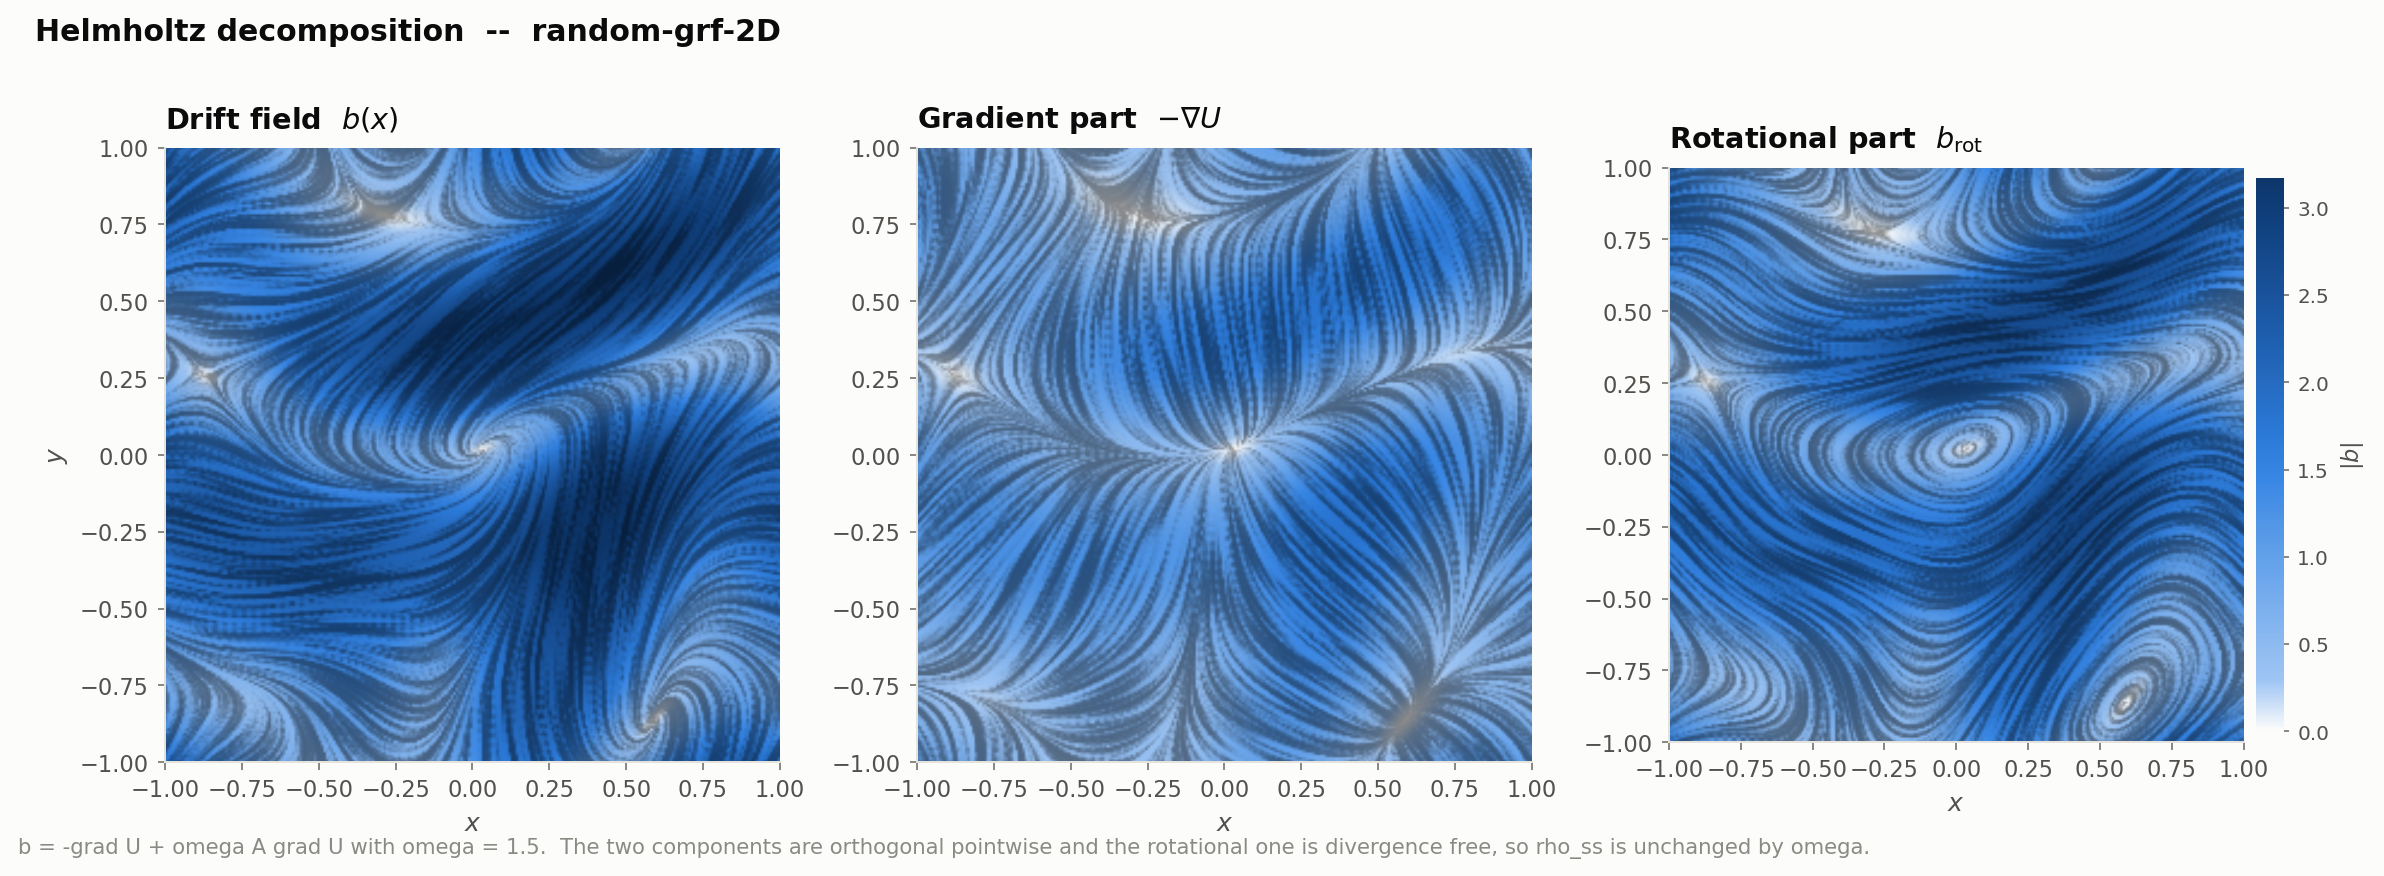
\includegraphics[width=\textwidth]{figs/helmholtz.png}
\caption{The decomposition of Eq.~\eqref{eq:construction} at $\omega=1.5$, drawn with
line-integral-convolution texture. Left: the full drift. Middle: the gradient part,
with a visible source/sink at the origin. Right: the rotational part, circulating.
All three share one speed scale.}
\end{figure}

\subsection{Field constructors}

\begin{center}
\begin{tabular}{@{}L{0.30\textwidth} L{0.10\textwidth} L{0.52\textwidth}@{}}
\toprule
\textbf{Constructor} & \textbf{Dim} & \textbf{What it is} \\
\midrule
\code{random\_grid\_field} & $d\le3$ &
  Potential on a periodic grid; spectral derivatives, quintic-spline interpolation.
  The backend you \emph{draw and animate}. \\
\code{random\_spectral\_field} & any $d$ &
  Random Fourier features $U=\sum_m a_m\cos(w_m\!\cdot\!x+\phi_m)$. Mesh-free, analytic
  derivatives, runs on GPU. The backend for the $d$-sweep. \\
\code{ornstein\_uhlenbeck} & any $d$ &
  $b=-kx$ (optionally $+\,\omega Ax$). Closed-form everything. \emph{Validate here first.} \\
\code{coupled\_ou\_chain} & any $d$ &
  Harmonically coupled chain, $K = kI + cL$. Stiff spectrum, pure gradient. \\
\code{DoubleWell1D} & 1 &
  $U = ax^4 - bx^2$. Metastable, non-Gaussian, gradient. \\
\code{RadialRotational2D} & 2 &
  Radial $U$ plus $\omega(-y,x)$. Textbook identifiability demonstrator. \\
\bottomrule
\end{tabular}
\end{center}

\subsubsection*{Key parameters}

\begin{center}
\begin{tabular}{@{}L{0.22\textwidth} L{0.13\textwidth} L{0.57\textwidth}@{}}
\toprule
\textbf{Parameter} & \textbf{Default} & \textbf{Meaning and effect} \\
\midrule
\code{d}                  & 2       & Dimension. Grid backend dies above 3 ($n^d$ cells). \\
\code{resolution}         & 256     & Grid points per axis (grid backend). \\
\code{n\_features}        & 256     & Fourier modes $M$ (spectral backend); 256\textendash{}1024 is plenty to $d=10$. \\
\code{omega}              & 0.0     & Rotational strength. $0$ = equilibrium; $1$ = equal power in both parts. \\
\code{correlation\_length}& $L/5$   & Feature size. Sets the gradient scale $\ell$. \\
\code{drift\_scale}       & 1.0     & Rescales $U$ so that $\mathrm{RMS}|b|$ equals this. Fixes units. \\
\code{seed}               & None    & Reproducibility. \\
\code{generator}          & spectral& \code{'spectral'} (Gaussian random field) or \code{'perlin'} (fBm). \\
\code{kernel}             & gaussian& \code{'gaussian'} (RBF) or \code{'matern'} (rougher), spectral backend. \\
\code{box}                & torus   & \code{Box.cube(d, 1.0, periodic=True)} by default. \\
\bottomrule
\end{tabular}
\end{center}

\subsubsection*{Noise spectra (grid backend)}

\begin{center}
\begin{tabular}{@{}L{0.16\textwidth} L{0.30\textwidth} L{0.46\textwidth}@{}}
\toprule
\textbf{\code{spectrum}} & \textbf{$P(k)$} & \textbf{Character} \\
\midrule
\code{'gaussian'}  & $e^{-(k\ell)^2/2}$ & \textbf{Default.} One smooth scale, all derivatives governed by $\ell$, resolution-independent. \\
\code{'powerlaw'}  & $(1+(k\ell)^2)^{-s/2}$ & Multi-scale / fBm-like. Use $s\ge6$ in 2D \textemdash{} see the warning below. \\
\code{'bandpass'}  & shell at $k_0$ & Cellular, wave-like structure. \\
\bottomrule
\end{tabular}
\end{center}

\begin{warnbox}
\textbf{Why the default is Gaussian, not power-law.} With $s=4$ in 2D the variance of
the \emph{second} derivatives goes like $\int k^3 P(k)\,\mathrm{d}k$, which diverges
logarithmically. The field's gradient scale $\ell = |b|/|\nabla b|$ is then set by
wherever the band limit happens to sit, not by \code{correlation\_length}. Measured:
$\ell$ fell from $0.055$ to $0.033$ when the grid was refined $128\to256$ \textemdash{}
i.e. the ``ground truth'' depended on grid resolution, and carried real structure at
scales no estimator could ever resolve. A Gaussian spectrum cuts off exponentially and
held $\ell \approx 0.24$ at both resolutions.
\end{warnbox}

\subsection{Domains}

\code{Box(lo, hi, periodic)} with helpers \code{Box.cube(d, half\_width, periodic)} and
\code{Box.unit(d, length, periodic)}. Boundary modes for simulation: \code{'periodic'}
(wrap), \code{'reflecting'} (mirror), \code{'none'} (open).

\begin{keybox}
\textbf{The torus is the default, and \code{Box.displacement} is why it works.}
On a periodic box no walker escapes and the whole domain gets sampled, which removes
the empty-tail-bin pathology from the estimator comparison. The cost is one piece of
bookkeeping, done in exactly one place: a walker that steps off the right edge
reappears on the left, so the raw difference $x_{t+1}-x_t$ is a box-sized jump. The
minimum-image convention returns the shortest representative instead. \emph{Every}
increment in the project goes through \code{Box.displacement}.
\end{keybox}

\subsection{Trajectories: \code{simulate()}}

\begin{center}
\begin{tabular}{@{}L{0.20\textwidth} L{0.13\textwidth} L{0.59\textwidth}@{}}
\toprule
\textbf{Parameter} & \textbf{Default} & \textbf{Meaning} \\
\midrule
\code{n\_walkers}  & 256   & $N$ independent walkers. \\
\code{n\_steps}    & 1000  & $T$ recorded transitions ($T+1$ frames). \\
\code{dt}          & 0.01  & \textbf{Observation} interval \textemdash{} the spacing of recorded frames. \\
\code{D}           & 0.05  & Diffusion coefficient; noise amplitude $\sqrt{2D\,\mathrm{d}t}$. \\
\code{substeps}    & 1     & Euler sub-steps per recorded interval (integration at $\mathrm{d}t/k$). \\
\code{burn\_in}    & 0.0   & Time run and discarded, so frames come from the stationary state. \\
\code{x0}          & None  & \code{None} (uniform on torus), a point \code{(d,)} (all together \textemdash{} the spreading-cloud run), an array \code{(N,d)}, or \code{'stationary'}/\code{'uniform'}/\code{'center'}. \\
\code{obs\_noise}  & 0.0   & Per-coordinate measurement noise added to recorded positions. \\
\code{boundary}    & auto  & \code{'periodic'}, \code{'reflecting'}, \code{'none'}. \\
\code{backend}     & numpy & \code{'numpy'} or \code{'torch'} (GPU; needs \code{field.supports\_torch}). \\
\code{torch\_dtype}& float32 & float32 is $\sim2\times$ faster on consumer GPUs. \\
\code{store\_dtype}& float32 & Storage precision; integration is always float64. \\
\bottomrule
\end{tabular}
\end{center}

\begin{keybox}
\textbf{Two different $\Delta t$'s, and confusing them ruins the bias experiment.}
\code{dt} is what the \emph{observer} sees; \code{dt/substeps} is what the
\emph{integrator} uses. With \code{substeps=1} an $O(\Delta t)$ error in the estimator
is indistinguishable from an $O(\Delta t)$ error in the simulator, and you would be
measuring your own integrator. Simulate with \code{substeps} large, observe at
\code{dt}, and the bias you plot is the estimator's.
\end{keybox}

\subsubsection*{Step-size diagnostics}

\code{suggest\_dt(field, D)} returns the largest $\Delta t$ meeting three criteria at
once; \code{check\_step(field, dt, D)} reports them:

\begin{center}
\begin{tabular}{@{}L{0.22\textwidth} L{0.22\textwidth} L{0.48\textwidth}@{}}
\toprule
\textbf{Key} & \textbf{Quantity} & \textbf{Want} \\
\midrule
\code{drift\_length\_scale} & $\ell = |b|/|\nabla b|$ & the field's own gradient scale \\
\code{drift\_cfl}     & $|b|\,\Delta t/\ell$          & $<0.1$ \\
\code{diffusive\_cfl} & $\sqrt{2dD\Delta t}/\ell$     & $<0.2$ \textemdash{} usually the binding one \\
\code{stability}      & $|\nabla b|\,\Delta t$        & $<0.1$; above $\sim1$ the run is nonsense \\
\code{ok}             & all three                     & \code{simulate} warns if \code{False} \\
\bottomrule
\end{tabular}
\end{center}

The diffusive criterion is the one people get wrong: a walker that diffuses a full
gradient scale per step steps straight \emph{over} the structure of $b$, and the
stationary density comes out visibly wrong even though the run looks perfectly stable.

\subsection{What a \code{Trajectories} object holds}

\begin{center}
\begin{tabular}{@{}L{0.24\textwidth} L{0.24\textwidth} L{0.44\textwidth}@{}}
\toprule
\textbf{Attribute} & \textbf{Shape / type} & \textbf{Notes} \\
\midrule
\code{.x}            & \code{(N, T+1, d)} & observed positions (noisy if \code{obs\_noise}$>0$) \\
\code{.x\_true}      & \code{(N, T+1, d)} & clean positions, kept only when noise was added \\
\code{.dt}, \code{.D}& float              & observation interval, diffusion coefficient \\
\code{.box}          & \code{Box}         & carries the periodicity increments need \\
\code{.dt\_integration} & float           & \code{dt/substeps} \\
\code{.n\_transitions}  & int             & $N\!\cdot\!T$ \textemdash{} the sample size that governs error \\
\code{.times}, \code{.duration} & array, float & \\
\bottomrule
\end{tabular}
\end{center}

\subsubsection*{Operations}

\begin{center}
\begin{tabular}{@{}L{0.34\textwidth} L{0.60\textwidth}@{}}
\toprule
\textbf{Method} & \textbf{Returns / purpose} \\
\midrule
\code{.increments()}                & \code{(N,T,d)} displacements, minimum-image corrected \\
\code{.pairs()}                     & \code{(x, dx)} flattened to \code{(N*T, d)} \textemdash{} the regression data \\
\code{.drift\_target()}             & \code{(x, dx/dt)} \textemdash{} the Kramers\textendash{}Moyal target \\
\code{.subsample\_time(k)}          & every $k$-th frame, $\Delta t\!\to\!k\Delta t$ \textemdash{} the $\Delta t$ sweep \\
\code{.subsample\_walkers(n)}       & the $N$ axis of a sweep \\
\code{.truncate(n\_frames)}         & the $T$ axis of a sweep \\
\code{.with\_observation\_noise($\sigma$)} & add measurement noise after the fact \\
\code{.msd()}                       & mean squared displacement per frame \\
\code{.step\_statistics()}          & dict: rms step vs pure-diffusion prediction, etc. \\
\code{.save() / .load()}            & compressed \code{.npz} round-trip \\
\bottomrule
\end{tabular}
\end{center}

\begin{keybox}
\code{subsample\_time} runs a $\Delta t$ sweep over the \emph{same underlying paths},
so differences across the sweep are pure estimator bias rather than a new realisation.
Simulate once, sweep for free.
\end{keybox}

\subsection{Snapshots}

\code{sample\_stationary(field, n, D, method=...)} returns \code{(n, d)} independent
draws from $\rho_{\mathrm{ss}}$ with \emph{no time ordering} \textemdash{} the input to
the density-only half of the project.

\begin{itemize}[leftmargin=1.4em,itemsep=1pt]
  \item \code{method='grid'} \textemdash{} samples the exact Boltzmann density on the
        field's own grid. Fast, no equilibration error. Verified to add no bias beyond
        the independent-sample floor.
  \item \code{method='dynamic'} \textemdash{} runs independent walkers past equilibrium
        and takes the final frame. Works for any field, including high $d$.
\end{itemize}

\subsection{Measurement noise}

Noise is applied \emph{after} simulation, which is the physically right order: the
walker follows the true dynamics and the microscope is what is imprecise.

\begin{warnbox}
\textbf{The $\sigma/\Delta t$ pathology.} Observation noise adds $2\sigma^2$ to the
increment variance \textemdash{} a term that does \textbf{not} vanish as
$\Delta t\to0$. The apparent drift $\Delta x/\Delta t$ therefore picks up a spurious
contribution $\sim\sigma/\Delta t$, so \emph{finer sampling makes things worse}. This is
the actual limiting factor in real single-particle-tracking data, and it is why
\code{obs\_noise} is a first-class sweep axis rather than an afterthought.
\end{warnbox}

\subsection{A field's own accessors}

Every field answers these, which is what makes the metrics exact:

\begin{center}
\begin{tabular}{@{}L{0.32\textwidth} L{0.62\textwidth}@{}}
\toprule
\textbf{Method} & \textbf{Returns} \\
\midrule
\code{.drift(x)}              & $b(x)$, shape \code{(...,d)} \\
\code{.potential(x)}          & $U(x)$ \\
\code{.grad\_potential(x)}    & $\nabla U(x)$ \\
\code{.gradient\_part(x)}     & $-\nabla U$ \\
\code{.rotational\_part(x)}   & $b + \nabla U$ \\
\code{.log\_rho\_ss(x, D)}    & $\log\rho_{\mathrm{ss}}$ up to a constant \\
\code{.score\_ss(x, D)}       & $\nabla\log\rho_{\mathrm{ss}}$ \\
\code{.stationary\_current(x, D)} & $J = b\rho - D\nabla\rho$; zero iff detailed balance \\
\code{.divergence(x)}         & $\nabla\!\cdot\!b$ (exact where available) \\
\code{.typical\_scale()}      & $\mathrm{RMS}|b|$ \textemdash{} the unit errors are reported in \\
\code{.concentration(D)}      & how tightly $\rho_{\mathrm{ss}}$ concentrates (see below) \\
\code{.with\_omega(w)}        & same $U$, different circulation \\
\code{.entropy\_production(D)}& $\sigma = \langle|b_{\mathrm{rot}}|^2\rangle/D$, by quadrature \\
\bottomrule
\end{tabular}
\end{center}

\begin{warnbox}
\textbf{Choose $D$ deliberately.} \code{field.concentration(D)} reports the density's
dynamic range. Below $\sim10$ the walkers cover the whole domain and the estimator
comparison is about the \emph{method}. Above $\sim1000$ they sit in one basin, most of
the field is never visited, and any ``error over the box'' is really a statement about
extrapolation. Picking $D$ by eye from a picture is how people end up comparing
estimators on data that never visited most of the field.
\end{warnbox}

% ==========================================================================
\clearpage
\section{Estimators}

\subsection{The contract}

Everything downstream \textemdash{} metrics, sweeps, phase diagrams \textemdash{} talks
to estimators only through this interface. Implement it and the entire comparison
machinery works on your method with no further wiring.

\begin{codebox}
\begin{lstlisting}
class TrajectoryEstimator(DriftEstimator):     # sees (x, dx): time ordering
    def fit(self, traj: Trajectories) -> Self: ...
    def predict(self, x) -> np.ndarray:        ...   # (..., d) in and out
    def support(self, x) -> np.ndarray:        ...   # where is it trustworthy?
    def uncertainty(self, x):                  ...   # optional: own error bar
    def predict_diffusion(self, x):            ...   # optional: D(x)

class SnapshotEstimator(DriftEstimator):       # sees positions only
    def fit(self, samples, D, box=None) -> Self: ...
    def predict_score(self, x) -> np.ndarray:    ...  # grad log rho_ss
    # predict() = D * predict_score(), so the equilibrium assumption
    # is written down in exactly one place instead of being smuggled in
\end{lstlisting}
\end{codebox}

Two helpers on the trajectory base class:
\code{self.regression\_data(traj)} gives $(x,\ \Delta x/\Delta t)$, and
\code{self.noise\_level(traj)} gives $\sqrt{2D/\Delta t}$ \textemdash{} the
per-coordinate noise on each raw target.

\begin{keybox}
\textbf{Why every rung is a form of local averaging.} The raw pointwise target
$\Delta x/\Delta t$ has standard deviation $\sqrt{2D/\Delta t}$, which for typical
settings is an \emph{order of magnitude larger} than $|b|$ itself. In the shipped demo,
$\mathrm{RMS}|b| = 1.0$ while $\mathrm{RMS}|\Delta x/\Delta t| = 17.5$. That is not a
defect to be fixed; it is the whole problem. Every method in the ladder differs only in
\emph{how} it averages that noise away.
\end{keybox}

\subsection{The ladder}

\begin{center}
\small
\begin{tabular}{@{}C{0.035\textwidth} L{0.235\textwidth} L{0.115\textwidth} L{0.105\textwidth} L{0.37\textwidth}@{}}
\toprule
\textbf{\#} & \textbf{Class} & \textbf{Key} & \textbf{Input} & \textbf{Expected behaviour} \\
\midrule
1 & \code{BinnedKramersMoyal} & \code{binned\_km} & trajectories &
  Cheapest, noisiest. Undefined in high $d$ ($\mathrm{bins}^d$ cells). \\
2 & \code{KernelRegression} & \code{kernel} & trajectories &
  Smooth weights; local-linear removes the density-gradient bias. \\
3 & \code{BasisProjection} & \code{sfi} & trajectories &
  \textbf{Expected winner in low $d$.} Closed form + analytic error bound. \\
4 & \code{NeuralDrift} & \code{nn} & trajectories &
  Should lose in $d\le2$; wins once the basis outgrows the data. \\
5a & \code{KDEScore} & \code{kde\_score} & snapshots &
  Recovers the gradient part only \textemdash{} by construction. \\
5b & \code{DenoisingScoreMatching} & \code{dsm} & snapshots &
  Same, learned. The diffusion-model hook. \\
\midrule
-- & \code{ZeroDrift} & \code{zero} & --- & \textcolor{aqua}{\textbf{Built.}} Null model; scores exactly $1.0$. \\
-- & \code{OracleDrift} & \code{oracle} & --- & \textcolor{aqua}{\textbf{Built.}} Truth; must score $\approx 0$. \\
\bottomrule
\end{tabular}
\end{center}

\subsection{Rung 1 \textemdash{} Binned Kramers\textendash{}Moyal}

\[
  \hat b(x) = \frac{1}{\Delta t}\,
  \frac{\sum_{i\in \mathrm{cell}(x)} \Delta x_i}{\#\{i\in \mathrm{cell}(x)\}} .
\]

Vectorise it: \code{np.ravel\_multi\_index} turns a $d$-dimensional cell address into a
flat one, then \code{np.bincount(flat, weights=dx[:,j])} sums each component in one
pass. The whole estimator is three lines; looping over cells is 100$\times$ slower.

\textbf{What to expect and report:} variance falling as $n(x)^{-1/2}$ per cell; an
$O(h^2)$ bias from averaging $b$ over a cell of width $h$; therefore a U-shaped total
error with an optimal bin count. In $d=6$ with 32 bins there are $10^9$ cells for maybe
$10^7$ samples \textemdash{} the estimator is not merely inaccurate but \emph{undefined},
which is the honest reason the ladder continues.

\subsection{Rung 2 \textemdash{} Kernel regression}

\[
  \hat b(x) = \frac{\sum_i K_h(x-x_i)\,\Delta x_i/\Delta t}{\sum_i K_h(x-x_i)} .
\]

That is Nadaraya\textendash{}Watson; \code{local\_linear=True} instead fits a local
linear model by weighted least squares and keeps the constant term.

\textbf{Why the local-linear variant matters.} Nadaraya\textendash{}Watson is badly
biased wherever the sample density has a strong gradient: the kernel pulls in more
samples from the dense side, dragging the average toward that side's drift value. Since
the density here is $e^{-U/D}$, its gradient is largest exactly on the slopes where the
drift is largest. Local-linear fitting cancels that term. Demonstrating this on the
double well, where the density gradient is savage, is a genuinely good result.

\textbf{Speed.} Naive evaluation is $O(n_{\mathrm{query}}\,n_{\mathrm{samples}})$. Use a
\code{cKDTree} with radius $\sim3h$, or bin to a fine grid and convolve with
\code{gaussian\_filter} \textemdash{} the latter turns the estimator into two
convolutions and is exact for gridded queries.

\subsection{Rung 3 \textemdash{} Basis projection (Stochastic Force Inference)}

Expand $b_j(x) = \sum_a c_{ja} f_a(x)$ and solve by least squares against the same
Kramers\textendash{}Moyal targets:
\[
  C = (F^{\mathsf T}F)^{-1} F^{\mathsf T} Y , \qquad Y = \Delta x/\Delta t .
\]
Every increment informs every coefficient, so instead of dividing the data among bins
you use all of it for each unknown. Reference: Frishman \& Ronceray, \emph{Phys.\ Rev.\
X} \textbf{10}, 021009 (2020).

\begin{keybox}
\textbf{Implement the information bound \textemdash{} it is the best part.} The method
estimates its own error from the data alone, with no ground truth:
\[
  \big\langle |\hat b - b|^2 \big\rangle \;\approx\;
  \frac{n_{\mathrm{basis}}\; d\; D}{n\,\Delta t} \;+\; (\text{projection bias}) .
\]
This turns ``my error is 4\%'' into ``my error is 4\%, the theory says 3.7\%, and here
they are on the same axes across three decades of sample size''. An error bar that needs
no ground truth is what makes a method usable on real data.
\end{keybox}

\textbf{Bases.} Polynomial (degree 1 spans OU \emph{exactly} \textemdash{} the ideal
validation case); Fourier (natural on the torus, and the random fields \emph{are}
band-limited sums of exactly this form, so the bias term is genuinely zero); RBF.

\textbf{The curse, quantified.} Polynomials of degree $p$ in $d$ dimensions number
$\binom{d+p}{p}$: at $p=3$, $d=2$ gives 10 but $d=10$ gives 286. Fourier is far worse,
$(2n_{\max}+1)^d$. Since the variance term grows linearly in $n_{\mathrm{basis}}$,
\textbf{this is the crossover the phase diagram is looking for}.

\subsection{Rung 4 \textemdash{} Neural network regression}

An MLP $x\mapsto b(x)$ trained on the same target. There is no trick. The question is
not \emph{can} a network do this (it can) but \emph{where it starts to be worth it}.

\begin{warnbox}
\textbf{Do not judge convergence by the loss.} The squared loss is dominated by the
irreducible noise floor $2dD/\Delta t$ and barely moves even as the fit improves.
\code{self.noise\_floor(traj)} returns it; plot the \emph{excess} over it, or the curve
looks flat from epoch one and tells you nothing.
\end{warnbox}

Other things that decide whether this works: standardise inputs \emph{and} targets
(targets are $10$\textendash$100\times$ larger than the drift); hold out whole
\emph{walkers}, not random timepoints (consecutive frames are correlated, so a random
split leaks); feed $[\sin(2\pi x/L), \cos(2\pi x/L)]$ on a torus or the network must
learn that the two edges are the same place and will show a seam; and sweep the implicit
smoothness (width, weight decay) or you are comparing a tuned method against an untuned
one.

\subsection{Rung 5 \textemdash{} Score-based, from snapshots}

The identity that makes this substantive rather than decorative:
\begin{equation}
  \nabla\log\rho_{\mathrm{ss}}(x) \;=\; -\nabla U(x)/D \;=\; b(x)/D
  \qquad\text{(gradient drift only).}
\end{equation}
A denoising score-matching model trained on snapshots is not a black box borrowed from
generative modelling; it is estimating precisely the physical quantity we want.

\textbf{KDE score} has a closed-form gradient, so no numerical differentiation is
needed:
$\nabla\log\hat\rho(x) = -h^{-2}\sum_i w_i (x-x_i)\big/\sum_i w_i$. Use
\code{box.displacement} for the offsets or the estimate is wrong near the edges. The
interesting catch: the optimal bandwidth for estimating $\rho$ is too small for
estimating $\nabla\log\rho$, and in the tails the log-gradient is dominated by the few
samples that happen to be there.

\textbf{Denoising score matching} minimises
$\mathbb{E}\big[\,|s_\theta(\tilde x,\sigma) + (\tilde x - x)/\sigma^2|^2\,\big]$ with
$\tilde x = x + \sigma\epsilon$. Evaluate at the \emph{smallest} $\sigma$ in the
training range. Here $\sigma$ plays the role of diffusion time in a generative model:
training this is the same computation as training a diffusion model on the snapshot
dataset \textemdash{} the only difference is that we want the score itself rather than
samples from it.

\begin{keybox}
\textbf{Then run it on a rotational system and watch it fail \textemdash{} as it must.}
Both snapshot methods return the gradient part with the rotational part missing, for
every $\omega$. That confirmation is the point of the whole rung.
\end{keybox}

% ==========================================================================
\clearpage
\section{Measuring and comparing}

\subsection{Where you evaluate matters more than the metric}

\code{make\_eval\_set(field, D, measure=...)} makes the choice explicit and records it:

\begin{itemize}[leftmargin=1.4em,itemsep=1pt]
  \item \code{'stationary'} \textemdash{} points drawn from $\rho_{\mathrm{ss}}$. The
        default and the honest one: it scores a method where the data actually is.
  \item \code{'uniform'} \textemdash{} uniform on the box. Harsher. \textbf{The gap
        between the two \emph{is} the extrapolation penalty.}
\end{itemize}

Pass \code{traj=} and each evaluation point also carries the training data's local
density, which is what \code{error\_vs\_density} bins against.

\subsection{What \code{drift\_error} returns}

\begin{center}
\begin{tabular}{@{}L{0.21\textwidth} L{0.73\textwidth}@{}}
\toprule
\textbf{Key} & \textbf{Meaning} \\
\midrule
\code{nrmse}      & $\mathrm{RMS}|\hat b - b| / \mathrm{RMS}|b|$. \textbf{The headline number.} $0$ perfect, $1$ = as good as predicting zero. \\
\code{nrmse\_grad}& error in the \emph{gradient} direction, normalised by that component \\
\code{nrmse\_rot} & error in the \emph{rotational} direction \\
\code{nrmse\_perp}& residual, off both structure directions \\
\code{cosine}     & mean alignment. Separates ``right shape, wrong scale'' from ``wrong shape'' \\
\code{scale\_ratio}& $\mathrm{RMS}|\hat b|/\mathrm{RMS}|b|$. Below 1 = over-smoothing \\
\code{supported\_fraction} & fraction of points the estimator claims to cover \\
\bottomrule
\end{tabular}
\end{center}

\begin{keybox}
\textbf{Normalisation is what makes the numbers mean something.} Because everything is
divided by $\mathrm{RMS}|b|$, \code{nrmse = 1.0} means ``learned nothing''. Methods
genuinely do score \emph{above} 1 at small sample sizes, and a reader cannot tell
without the null line \textemdash{} which is why \code{ZeroDrift} is drawn on every plot.

\textbf{Diagnostics for free.} A low \code{cosine} means the shape is wrong; a
\code{scale\_ratio} far from 1 usually means a missing $1/\Delta t$ or a factor of 2 in
$D$. Those two catch most first-attempt bugs.
\end{keybox}

\subsection{The error decomposition}

Because the two parts of Eq.~\eqref{eq:construction} are orthogonal \emph{pointwise},
the error vector splits exactly along the field's own structure:
\[
  \hat b - b \;=\; e_{\mathrm{grad}}\,\hat g \;+\; e_{\mathrm{rot}}\,\hat r \;+\; e_\perp ,
  \qquad
  \hat g = \frac{\nabla U}{|\nabla U|},\quad
  \hat r = \frac{A\nabla U}{|A\nabla U|} .
\]

This is what turns the identifiability claim into two numbers. A method that recovers
the potential perfectly but misses the circulation entirely \textemdash{} which is what
\emph{every} snapshot method must do \textemdash{} shows $e_{\mathrm{grad}}\approx0$ and
$e_{\mathrm{rot}}$ equal to the full rotational amplitude. That is a diagnosis, not just
an error bar.

\subsection{Sweeps}

\code{sweep\_grid(**axes)} takes the Cartesian product of named axes into a list of
\code{SweepConfig}s; \code{run\_sweep(configs, estimators, cache=...)} runs them and
returns a tidy \code{DataFrame}, one row per (config, estimator).

\begin{center}
\begin{tabular}{@{}L{0.20\textwidth} L{0.10\textwidth} L{0.62\textwidth}@{}}
\toprule
\textbf{Axis} & \textbf{Default} & \textbf{What it sweeps} \\
\midrule
\code{d}          & 2     & dimension (grid backend $\le3$, spectral above) \\
\code{n\_walkers} & 512   & $N$ \\
\code{n\_steps}   & 2000  & $T$ \\
\code{dt}         & None  & observation interval (\code{None} = \code{suggest\_dt}) \\
\code{D}          & 0.3   & diffusion coefficient \\
\code{omega}      & 0.0   & rotational strength \textemdash{} the identifiability axis \\
\code{obs\_noise} & 0.0   & measurement noise \\
\code{substeps}   & 1     & integration accuracy at fixed observation \code{dt} \\
\code{seed}       & 0     & \textbf{include several} \textemdash{} one seed is a number with no uncertainty \\
\code{measure}    & stationary & evaluation measure \\
\bottomrule
\end{tabular}
\end{center}

Three properties that keep the comparison honest: all estimators see exactly the same
data within a config and are scored on the same points; snapshot estimators get a
\emph{matched observation budget} ($N\!\cdot\!T$ independent samples, the generous
reading); and an estimator whose \code{fit} raises \code{NotImplementedError} yields a
row with \code{status='not\_implemented'} and the sweep continues. Results are cached by
config hash, so runs resume and adding a new estimator does not recompute trajectories.

% ==========================================================================
\clearpage
\section{Figures and animations}

Everything shares one design system (\code{dfi/viz/style.py}): a single-hue sequential
blue ramp for magnitudes, diverging blue$\leftrightarrow$red with a neutral grey
midpoint for signed quantities, a fixed categorical order for method identity, and a
light/dark theme switch (\code{use\_style('light'|'dark')}).

\begin{center}
\begin{tabular}{@{}L{0.30\textwidth} L{0.64\textwidth}@{}}
\toprule
\textbf{Function} & \textbf{Draws} \\
\midrule
\multicolumn{2}{@{}l}{\itshape\color{ink2} Fields} \\
\code{plot\_drift}        & the field, as LIC texture / streamlines / quiver \\
\code{plot\_potential}    & $U$ heatmap with contours (diverging ramp, zero at grey) \\
\code{plot\_density}      & $\rho_{\mathrm{ss}}$, exact or empirical \\
\code{plot\_helmholtz}    & the three-panel decomposition, shared colour scale \\
\code{plot\_field\_card}  & four-panel identity card: drift, $U$, $\rho$, power spectrum \\
\code{plot\_field\_1d}    & drift, potential and density for 1D systems \\
\midrule
\multicolumn{2}{@{}l}{\itshape\color{ink2} Trajectories} \\
\code{plot\_trajectories} & paths over the field, colour ramping with time \\
\code{plot\_snapshot}     & the unordered scatter \\
\code{plot\_sampling\_density} & \textbf{where the data actually is} \\
\code{plot\_msd}          & MSD against the free-diffusion line \\
\code{plot\_increment\_check} & increments vs $\mathcal{N}(0, 2D\Delta t)$ \\
\code{plot\_trajectories\_1d} & $x$ vs $t$ beside the occupancy histogram \\
\midrule
\multicolumn{2}{@{}l}{\itshape\color{ink2} Comparison} \\
\code{plot\_error\_curves}& error vs any sweep axis, with null line and slope guide \\
\code{plot\_identifiability} & gradient vs rotational error against $\omega$ \\
\code{plot\_phase\_diagram}  & which method wins over (budget, $d$), with crossover \\
\code{plot\_error\_vs\_density} & error against local sample density \\
\code{plot\_bias\_variance}  & the U-shape against a smoothing parameter \\
\code{plot\_training\_curve} & NN loss \emph{relative to the noise floor} \\
\midrule
\multicolumn{2}{@{}l}{\itshape\color{ink2} Animations (mp4 via ffmpeg, gif via Pillow)} \\
\code{animate\_diffusion} & walkers with fading trails and glowing heads \\
\code{animate\_omega\_sweep} & $\omega$ rising while $\rho_{\mathrm{ss}}$ refuses to move \\
\code{animate\_relaxation}& a point source spreading into $\rho_{\mathrm{ss}}$ \\
\bottomrule
\end{tabular}
\end{center}

\begin{keybox}
\code{plot\_sampling\_density} is the one people skip and shouldn't. A
Kramers\textendash{}Moyal estimate is a local average, so its variance at $x$ scales
like $1/n(x)$, and the regions where a method appears to ``fail'' are usually just the
regions nothing visited. Plotting error without plotting sample density beside it
invites the wrong conclusion.
\end{keybox}

\begin{figure}[h]
\centering
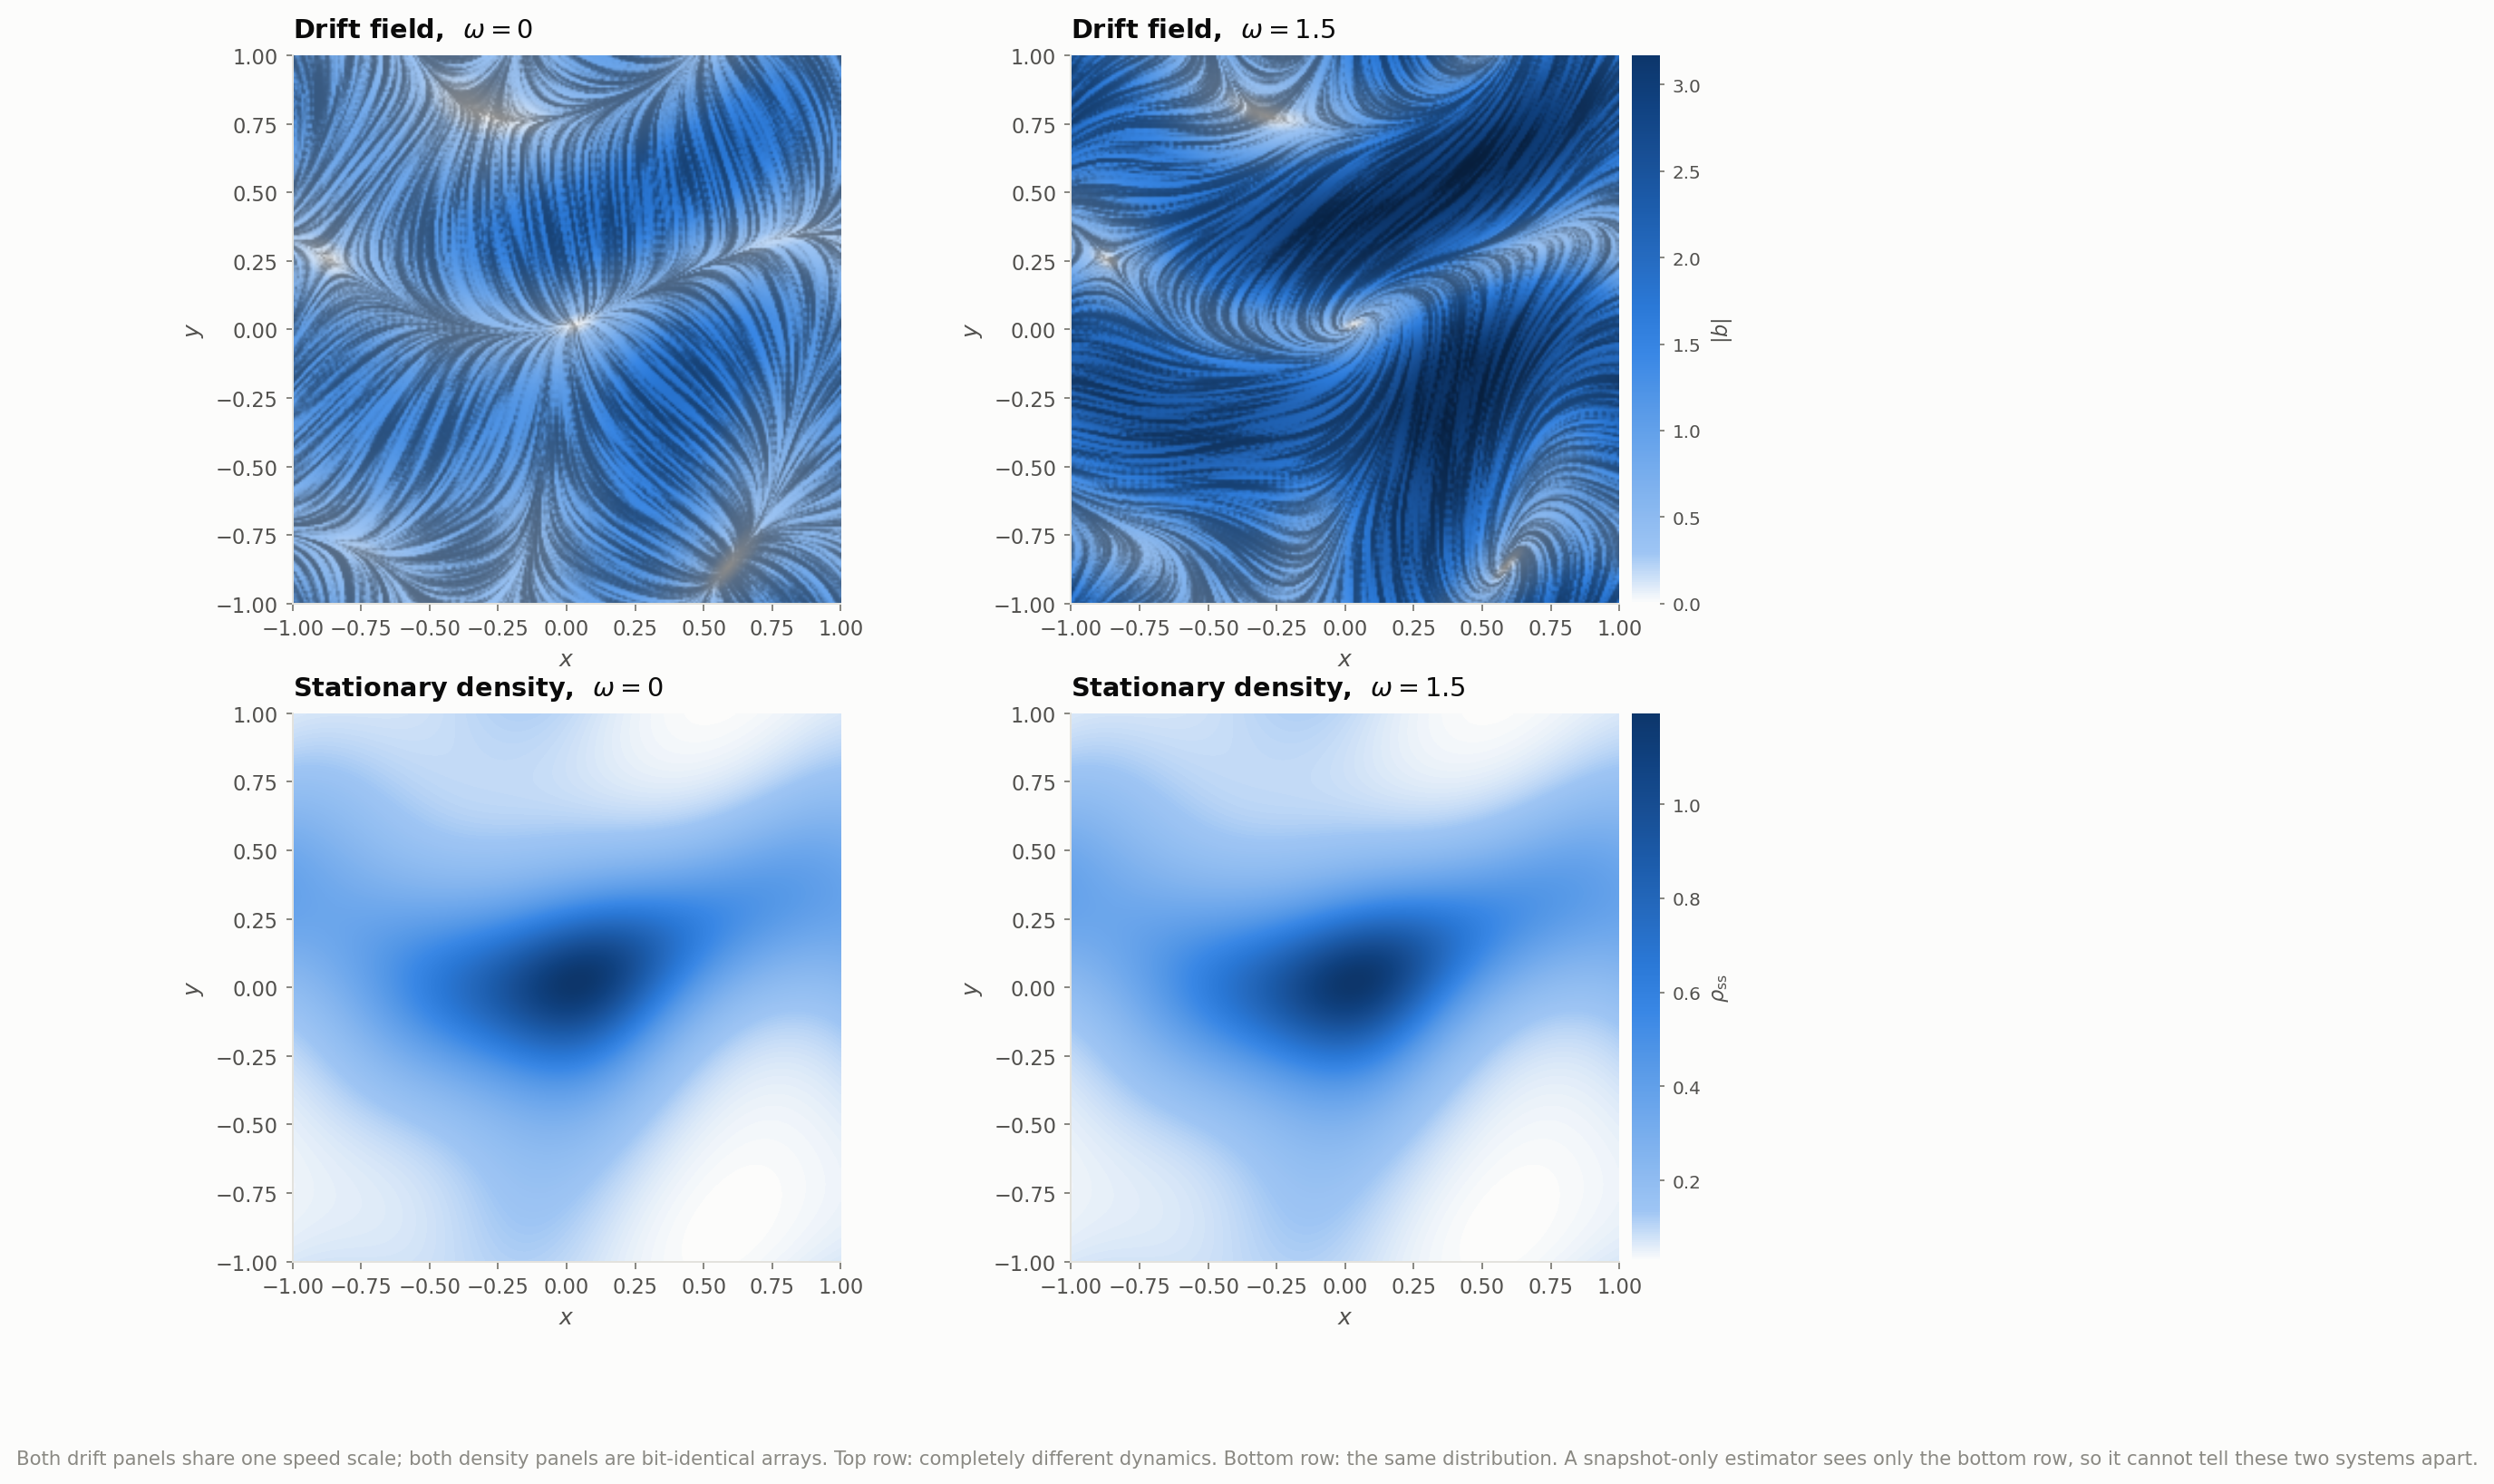
\includegraphics[width=0.85\textwidth]{figs/identifiability_static.png}
\caption{The headline figure. Both drift panels share one speed scale; both density
panels are bit-identical arrays. Top row: completely different dynamics. Bottom row: the
same distribution. A snapshot-only estimator sees only the bottom row.}
\end{figure}

% ==========================================================================
\clearpage
\section{Design decisions, and the measurements behind them}

\begin{center}
\begin{tabular}{@{}L{0.26\textwidth} L{0.68\textwidth}@{}}
\toprule
\textbf{Decision} & \textbf{Why, with the number} \\
\midrule
Scalar construction, Eq.~\eqref{eq:construction}
  & Exact Helmholtz split and exact Boltzmann density for every $\omega$.
    Fokker\textendash{}Planck residual: $2\times10^{-7}$. \\
Quintic B-splines, band limit at $0.25$ Nyquist
  & Ground-truth drift error $7\times10^{-6}$ relative. Cubic at the same band limit
    gives $5\times10^{-4}$; a $0.55$ band limit gives $3\times10^{-3}$. The estimators
    being benchmarked have percent-level errors, so the truth must be orders of
    magnitude tighter. \\
Gaussian spectrum by default
  & Power-law $s=4$ made $\ell$ fall $0.055\to0.033$ when the grid refined
    $128\to256$ \textemdash{} a resolution-dependent ground truth. Gaussian holds
    $\ell\approx0.24$ at both. \\
Observation \code{dt} $\ne$ integration step
  & So the measured $O(\Delta t)$ bias is the estimator's, not the integrator's. \\
Periodic torus + minimum image
  & Whole domain sampled; no empty-tail-bin pathology confounding the comparison. \\
Spectral tensor backend for $d>3$
  & A grid is $n^d$. Random Fourier features are mesh-free with analytic derivatives. \\
float32 on GPU
  & $d=8$, $N=40\,000$: numpy $258\,$s vs torch fp32 $13.2\,$s (\textbf{19.6$\times$}).
    fp32 is $\sim2\times$ faster than fp64 on consumer GPUs, at a rounding error five
    orders of magnitude below the diffusive step. \\
\bottomrule
\end{tabular}
\end{center}

\subsection{Validation already performed}

The scaffolding was checked end-to-end with throwaway estimators (kept out of the
repository \textemdash{} the real ones are yours). Everything landed on theory:

\begin{center}
\begin{tabular}{@{}L{0.38\textwidth} L{0.28\textwidth} L{0.28\textwidth}@{}}
\toprule
\textbf{Check} & \textbf{Expected} & \textbf{Measured} \\
\midrule
Error scaling with sample budget & ratio $2.00$ per $4\times$ data & $2.08,\ 1.92,\ 2.03$ \\
Error vs local sample density    & slope $-0.5$                    & $-0.477$ \\
Bias\textendash{}variance in bin width & U-shape                   & minimum at 8 bins \\
Oracle estimator                 & $0$                             & $<10^{-12}$ \\
Null estimator                   & $1.0$                           & $1.0000$ \\
Snapshot method, gradient error  & constant in $\omega$            & $0.176962$ at \emph{every} $\omega$ \\
Snapshot method, rotational error& exactly $1.0$                   & $1.0068,\ 1.0016,\ 1.0007$ \\
\bottomrule
\end{tabular}
\end{center}

\begin{figure}[h]
\centering
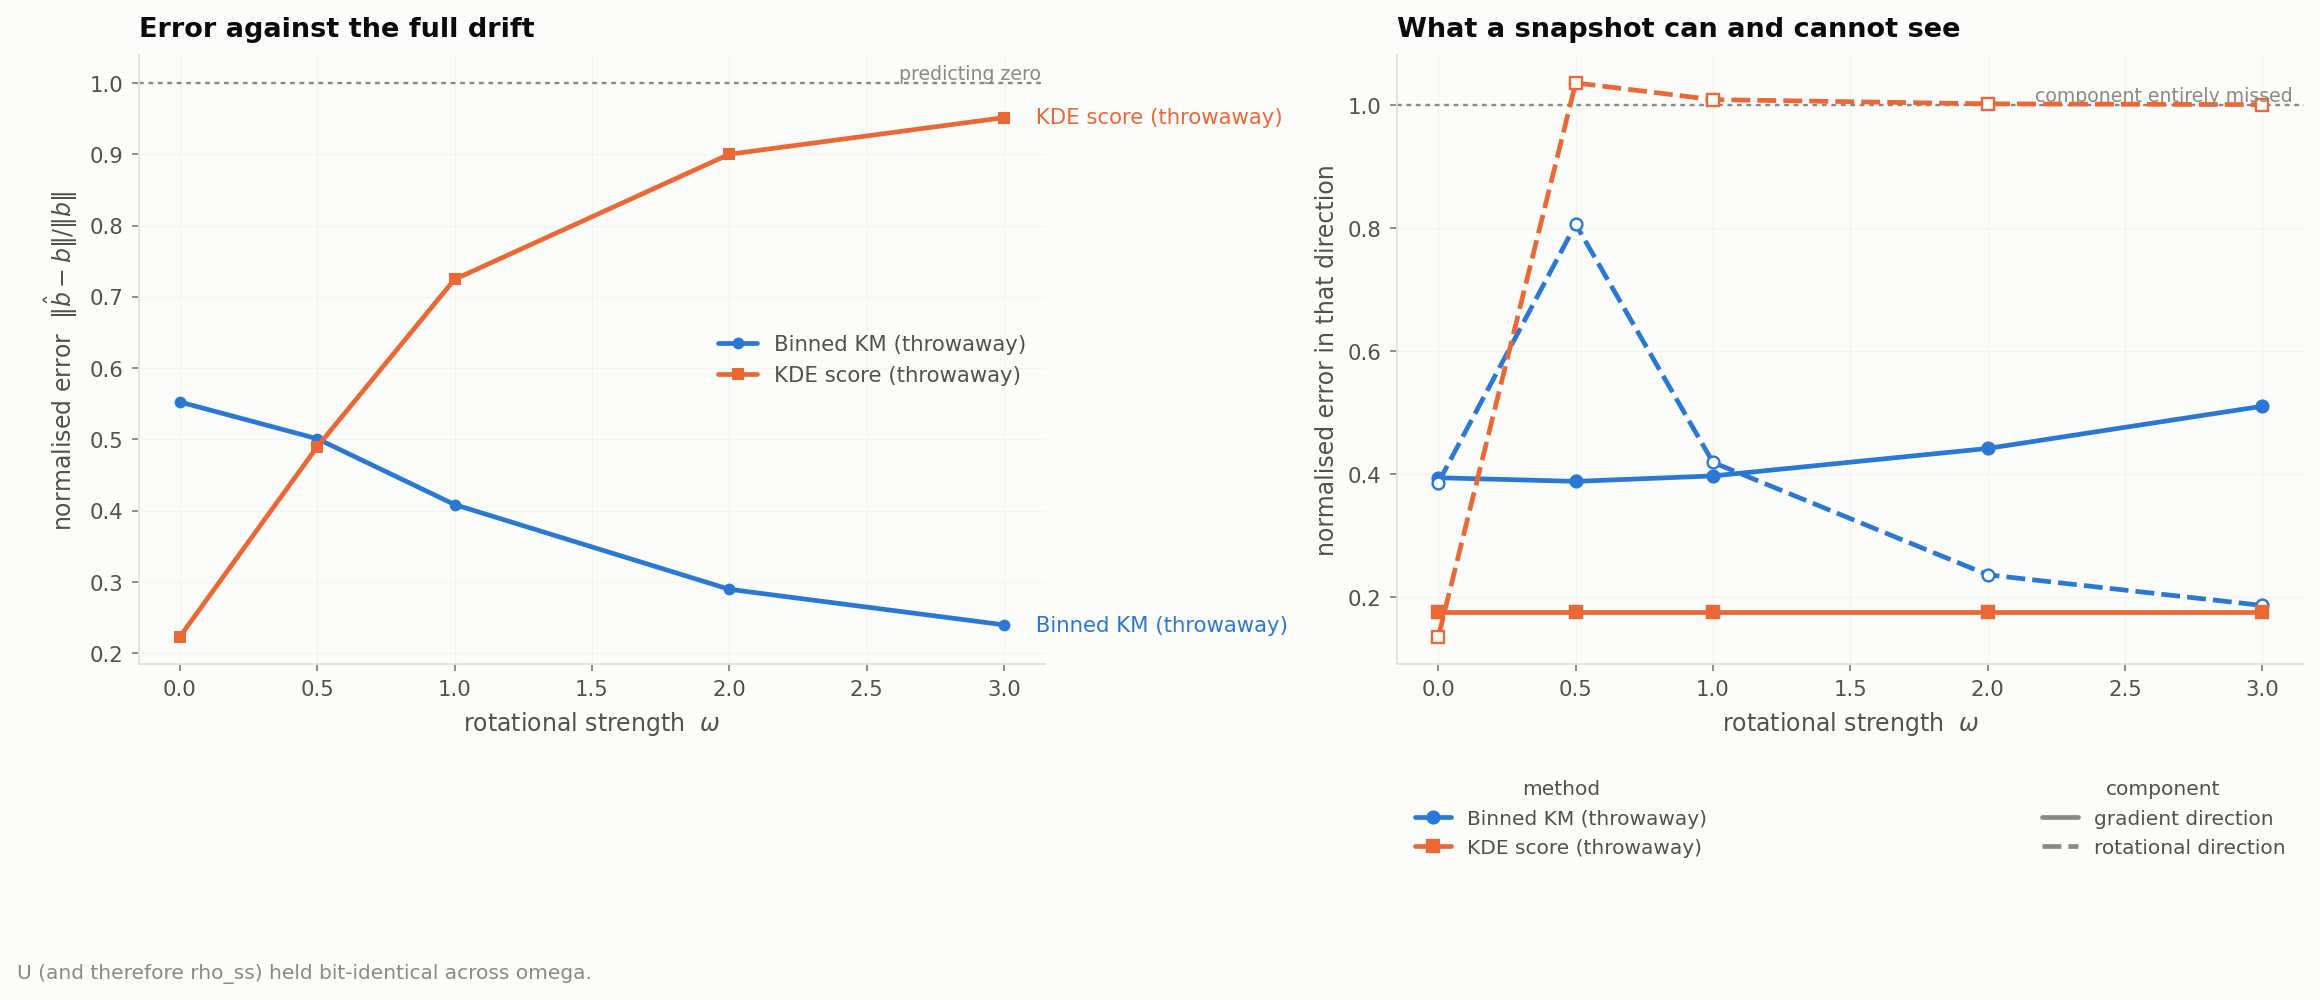
\includegraphics[width=\textwidth]{figs/identifiability_curves.png}
\caption{The identifiability result, produced by the built harness. Left: the snapshot
method climbs toward the null line as circulation grows, while the trajectory method
improves. Right: the decomposition \textemdash{} the snapshot method's
gradient-direction error is flat and its rotational-direction error is pinned at
$1.0$, meaning it misses \emph{exactly} 100\% of the circulation.}
\end{figure}

\begin{warnbox}
\textbf{A lesson worth keeping.} Three separate test ``failures'' during the build were
tolerances set below the Monte Carlo standard error, not bugs. The MSD estimator's
relative standard error is $\sqrt{2/N}$ \emph{independent of $t$} \textemdash{} 2.6\% at
$N=3000$. Derive test tolerances from the sample size; do not guess them.
\end{warnbox}

% ==========================================================================
\clearpage
\section{Cheat sheet}

\subsection*{End to end, today}

\begin{codebox}
\begin{lstlisting}
from dfi import (random_grid_field, random_spectral_field, simulate,
                 sample_stationary, suggest_dt, check_step)
from dfi.metrics import make_eval_set, drift_error, error_vs_density
from dfi.viz import use_style, plot_drift, plot_helmholtz, plot_trajectories

use_style("light")                          # or "dark"

# 1. a random field on a periodic torus
field = random_grid_field(d=2, resolution=256, omega=1.5, seed=0,
                          correlation_length=0.45, drift_scale=1.0)
print(field.summary(), field.concentration(D=0.3))

# 2. check the step, then simulate
D  = 0.3
dt = suggest_dt(field, D)
print(check_step(field, dt, D))
traj = simulate(field, n_walkers=2000, n_steps=4000, dt=dt, D=D,
                burn_in=10.0, substeps=1, seed=0)

# 3. the same potential without circulation -- rho_ss is bit-identical
equil = field.with_omega(0.0)

# 4. snapshots: positions only, no time ordering
snaps = sample_stationary(field, 200_000, D)

# 5. sweep axes for free, over the same underlying paths
coarse = traj.subsample_time(4)             # dt -> 4*dt
fewer  = traj.subsample_walkers(256)        # the N axis
noisy  = traj.with_observation_noise(0.01)  # the sigma axis

# 6. fit your estimator and score it
est = MyEstimator().fit(traj)
ev  = make_eval_set(field, D, n=20000, measure="stationary", traj=traj)
print(drift_error(est, field, ev))          # nrmse, nrmse_grad, nrmse_rot, ...
\end{lstlisting}
\end{codebox}

\subsection*{High dimension (GPU)}

\begin{codebox}
\begin{lstlisting}
field = random_spectral_field(d=8, n_features=512, omega=0.4, seed=0)
traj  = simulate(field, n_walkers=40_000, n_steps=2000,
                 dt=suggest_dt(field, 0.1), D=0.1,
                 backend="torch", torch_dtype="float32")   # 19.6x faster
\end{lstlisting}
\end{codebox}

\subsection*{Sweeps and figures}

\begin{codebox}
\begin{lstlisting}
from dfi.sweeps import sweep_grid, run_sweep
from dfi.viz.sweeps import plot_error_curves, plot_identifiability

cfgs = sweep_grid(d=2, n_walkers=[64, 256, 1024], n_steps=2000,
                  omega=[0.0, 1.0, 2.0], seed=[0, 1, 2])
df   = run_sweep(cfgs, {"mine": MyEstimator}, cache="outputs/data/sweep.csv")

plot_error_curves(df, x="n_transitions", y="nrmse")
plot_identifiability(df)
\end{lstlisting}
\end{codebox}

\subsection*{Scripts and tests}

\begin{center}
\begin{tabular}{@{}L{0.44\textwidth} L{0.50\textwidth}@{}}
\toprule
\textbf{Command} & \textbf{Does} \\
\midrule
\bt{python scripts/01\_fields\_and\_diffusion.py} & all static figures ($\sim1$ min) \\
\bt{\phantom{python scripts/01} ... {-}{-}animate} & plus mp4 animations ($\sim5$ min) \\
\bt{\phantom{python scripts/01} ... {-}{-}theme dark} & dark theme \\
\bt{python scripts/02\_sweeps.py {-}{-}quick} & sweep figures; works with baselines alone \\
\bt{pytest -q} & 28 tests; skips unimplemented rungs \\
\bt{pytest -q -k binned\_km} & one rung, verdict in $\sim2\,$s \\
\bottomrule
\end{tabular}
\end{center}

\vspace{1.2em}
\begin{keybox}
\textbf{Suggested order of work.} Implement \code{BinnedKramersMoyal.fit}, run
\code{pytest -q -k binned\_km} until it recovers $b(x)=-kx$ on 1D OU, then
\code{scripts/02\_sweeps.py {-}{-}quick} to see your first real curve. Work up the ladder
from there. Each rung is a genuine baseline for the next, and the negative results
\textemdash{} where the simple method wins \textemdash{} are the valuable output.
\end{keybox}

\end{document}
